\chapter{Studi Literatur}

Pada bab ini akan dipaparkan mengenai beberapa penelitian terkait deteksi intrusi paralel berbasis GPU yang telah dilakukan sebelumnya berikut metodologi serta ketercapaian yang didapatkan. Selain itu, pada bab ini juga akan dijelaskan lebih lanjut mengenai landasan teori dari pengerjaan tugas ini.

% Bab Studi Literatur digunakan untuk mendeskripsikan kajian literatur yang terkait dengan persoalan tugas akhir. Tujuan studi literatur adalah:
%
% \begin{enumerate}
%   \item menunjukkan kepada pembaca adanya gap seperti pada rumusan masalah yang memang belum terselesaikan,
%   \item memberikan pemahaman yang secukupnya kepada pembaca tentang teori atau pekerjaan terkait yang terkait langsung dengan penyelesaian persoalan, serta
%   \item menyampaikan informasi apa saja yang sudah ditulis/dilaporkan oleh pihak lain (peneliti/Tugas Akhir/Tesis) tentang hasil penelitian/pekerjaan mereka yang sama atau mirip kaitannya dengan persoalan tugas akhir.
% \end{enumerate}

\section{Intrusi}


  \subsection{Proses Intrusi Sistem}

    Intrusi merupakan serangkaian percobaan yang tidak berhak, baik sukses maupun tidak, untuk menyusup masuk, mengakses, mengubah, atau menyalahgunakan resource yang berharga sehingga resource menjadi tidak dapat diandalkan atau digunakan \parencite{kizza2015}.

    Proses intrusi sistem terbagi menjadi beberapa tahap. Proses dimulai dengan identifikasi target. Lalu target akan diperiksa secara menyeluruh dan dicari celah keamanannya. Selanjutnya mengambil akses ke sistem. Dan terakhir, mendapatkan akses, atau bahkan mengambil alih resource dalam sistem. 

    Umumnya proses pengambilan akses juga dapat dibagi menjadi 6 jenis:

    \begin{enumerate}
      \item Percobaan untuk menyusup
      \item Serangan dengan penyamaran
      \item Penetrasi terhadap sistem kontrol keamanan
      \item Kebocoran resource
      \item Penggunaan yang jahat, termasuk modifikasi dan perusakan resource sistem
    \end{enumerate}


    % \begin{enumerate}
    %   \item 
    %   Identifikasi target
    %   Proses ini bertujuan memetakan target yang akan diserang. 
    %   \item
    %   Pemeriksaan target
    %   Proses ini bertujuan memeriksa 
    %   \item
    %   Penyusupan ke dalam sistem
    %   Proses ini
    % \end{enumerate}  

  \subsection{Deteksi Intrusi}

    Deteksi intrusi adalah kegiatan merekam, menganalisa, dan mendeteksi kemungkinan sebuah percobaan akses yang tidak berhak terhadap sebuah sistem \parencite{kizza2015}. Adanya percobaan akses ilegal dapat mengindikasikan adanya serangan dari luar (seperti \emph{hijacking}, dst), maupun dari dalam (seperti \emph{malware}). Setelah serangan ditemukan, aktivitas akan dicatat ke log untuk ditindak lebih lanjut.

    Selain deteksi intrusi, kegiatan yang berkaitan adalah pencegahan intrusi. Pencegahan intrusi merupakan deteksi intrusi yang secara aktif melakukan penyaringan terhadap percobaan akses ke sistem. Jika terindikasi sistem terkena percobaan serangan, maka semua percobaan akses yang terkait akan dihentikan, atau lebih lanjut bisa diblok baik sementara waktu maupun secara permanen.

\section{Sistem Deteksi Intrusi}

  Sistem deteksi intrusi adalah mekanisme yang mengotomasi proses deteksi dan pencegahan serangan kepada satu atau beberapa node dalam suatu subnet jaringan. Sistem mengambil paket yang masuk sambil melakukan pengecekan kemudian membuat laporan hasil inspeksi. Laporan hasil inspeksi dapat digunakan untuk menentukan aksi yang akan dilakukan pada paket \parencite{nist2014}.

  \subsection{Metode Deteksi Intrusi}

    Ada tiga macam metode deteksi yang biasa dipakai dalam sistem deteksi intrusi:

    \begin{enumerate}

      \item
      \emph{Signature-based Detection}

      \emph{Signature} adalah pola aktivitas tertentu yang mengindikasikan adanya ancaman. Deteksi berbasis \emph{signature} adalah proses membandingkan \emph{signature} dengan aktivitas sistem untuk mengidentifikasi insiden yang mungkin. Pengenalan berbasis \emph{signature} sangat efektif dan cepat untuk mendeteksi ancaman yang telah dikenal tapi tidak efektif untuk mendeteksi ancaman yang belum dikenal sebelumnya atau ancaman yang disamarkan dengan teknik-teknik tertentu.

      Metode ini adalah metode termudah karena hanya membandingkan unit aktivitas saat ini, seperti paket atau \emph{log entry}, dengan daftar \emph{signature} menggunakan operasi perbandingan string. Metode berbasis \emph{signature} membutuhkan sedikit pengetahuan tentang protokol jaringan dan aplikasi, dan tidak dapat melacak atau mendapat state dari komunikasi yang kompleks.

      \item
      \emph{Anomaly-based Detection}

      Deteksi dengan anomali adalah proses membandingkan parameter aktivitas yang dianggap normal dengan aktivitas sistem sekarang untuk melihat penyimpangan yang signifikan. Sistem menggunakan profil untuk menentukan parameter aktivitas normal seperti user, host, koneksi jaringan, atau aplikasi. Profil dikembangkan menggunakan pembelajaran mesin dengan memantau karakteristik dari aktivitas sejenis selama selang waktu tertentu.

      Sistem akan menggunakan metode statistik untuk membandingkan karakteristik aktivitas sekarang terhadap batas yang terkait dengan profil. Ketika ada aktivitas yang menyimpang cukup jauh dari batas, akan dicatat ke \emph{log} dan dilaporkan ke \emph{administrator} / pengelola. Profil bisa dikembangkan dari berbagai atribut, seperti jumlah email yang dikirim oleh pengguna, jumlah percobaan login yang gagal, dan tingkat penggunaan CPU host waktu tertentu.

      Keuntungan dari metode berbasis anomali ini adalah dapat mendeteksi ancaman yang belum pernah dikenal sebelumnya. Contoh, sebuah proses yang menggunakan resource dalam jumlah besar, mengirim banyak email, menjalankan banyak koneksi, dan melakukan kegiatan lain yang cukup berbeda dari profil sistem normal akan terdeteksi sebagai \emph{malware}.

      Profil awal dibangkitkan selama rentang waktu tertentu yang disebut \emph{training period}. Kemudian profil dapat diperbarui secara statis atau dinamis. Dinamis ketika profil diperbarui dengan \emph{log} aktivitas sistem. Statis jika profil diperbarui secara manual.

      \item
      \emph{Stateful Protocol Analysis}

      \emph{Stateful protocol analysis} atau analisis protokol dengan \emph{state} adalah proses membandingkan profil yang telah ditentukan sebelumnya terhadap definisi aktivitas protokol yang dianggap tidak berbahaya yang berlaku umum untuk setiap protokol. Profil diukur terhadap batas tertentu untuk mengidentifikasi penyimpangan. 

      Tidak seperti deteksi berbasis anomali, yang menggunakan profil khusus host atau jaringan, analisis protokol dengan \emph{state} bergantung pada profil universal yang dikembangkan vendor yang menentukan bagaimana protokol tertentu seharusnya dan tidak boleh digunakan. Misalnya, saat pengguna memulai sesi File Transfer Protocol (FTP), sesi awalnya dalam \emph{state} yang tidak terotorisasi. Pengguna yang tidak terotorisasi hanya dapat melakukan beberapa perintah di \emph{state} ini, seperti melihat informasi umum dan memberikan nama pengguna dan kata sandi. 

      Bagian penting dari pemahaman \emph{state} adalah mencocokkan \emph{request} dengan respons, jadi ketika upaya otentikasi FTP terjadi, IDS dapat menentukan apakah berhasil dengan menemukan kode \emph{state} dalam respons yang sesuai. Setelah pengguna berhasil dikonfirmasi, sesi diset berada dalam keadaan terotentikasi, dan pengguna dapat melakukan lebih banyak perintah. Contohnya adalah jika terlalu banyak perintah dalam suatu \emph{request} dilakukan dalam \emph{state} yang tidak diotentikasi, maka akan dianggap mencurigakan. 

    \end{enumerate}

    Selain ketiga kategori diatas, penggunaan metode deteksi \emph{hybrid} \emph{signature-based} dan \emph{anomaly-based}. 

\section{\emph{Network Intrusion Detection and Prevention System}}

  \subsection{Snort NIDS}


\section{Pencocokan Pola}

  Salah satu komponen penting dalam pengecekan paket adalan pencocokan pola. Ada banyak jenis algoritma yang dapat digunakan untuk pencocokan pola. Salah satu algoritma yang paling banyak digunakan adalah algoritma Aho-Corasick. Algoritma ini dianggap cocok untuk deteksi intrusi karena dapat melakukan pengecekan multi pola.

  \subsection{Algoritma Aho-Corasick}

    Algoritma Aho-Corasick adalah salah satu algoritma untuk pencocokan string. Algoritma ini dapat mencari sebuah string dalam sebuah kumpulan string atau kamus \parencite{ahoc1975}. Pencarian juga bisa dilakukan pada substring terhadap semua string dalam kamus. Dengan memodelkan pola paket menjadi string atau regular expression, dapat dicari kemunculan pola serangan menggunakan algoritma Aho-Corasick ini.

    Kamus berisi semua string rule yang akan dicocokkan. Pembangkitan kamus hanya dilakukan sekali sebelum pencocokan string dilakukan. Ada beberapa desain kamus yang dapat digunakan. Salah satu bentuk yang umum yaitu \emph{finite automata} atau FSM (\emph{finite state machine}) yang menyerupai trie. 

    Trie adalah pohon yang menggambarkan urutan karakter prefiks dalam beberapa string \parencite{trie59}. Trie akan dimulai dari simpul kosong. Lalu bercabang hanya jika ada huruf yang berbeda. Sehingga pencarian string dalam kamus hanya dilakukan dengan menelusuri tiap simpul pada trie.

    Desain yang lebih padat menggunakan \emph{failure transition}. \emph{Failure transition} akan menunjuk ke posisi terakhir prefiks yang cocok dengan suffiks string yang dicari. Sehingga ketika pencarian tidak cocok pada suatu string, akan dilanjutkan pada string berikutnya yang prefiksnya cocok dengan suffiks string sebelumnya. Menggunakan \emph{failure function}, pencocokan banyak pola dapat lebih efisien ketimbang harus mengulang tiap pencarian dari awal. 

  % \subsection{\emph{Compressed Memory}}


\section{\emph{Compute Unified Device Architecture}}

  \emph{Compute Unified Device Architecture} 
  % (CUDA) adalah platform dan API () untuk komputasi paralel pada GPU. Platform CUDA hanya tersedia

  \subsection{\emph{CUDA Thread}}

  \subsection{\emph{Direct Memory Access}}

% \section{Dasar Teori}
% Perujukan literatur dapat dilakukan dengan menambahkan entri baru di berkas. Tulisan ini merujuk pada \parencite{parker1998} dan \parencite{4026885}

%   \subsection{Subbab}

%   \blindtext

%   \begin{figure}[h]
%     \centering
%     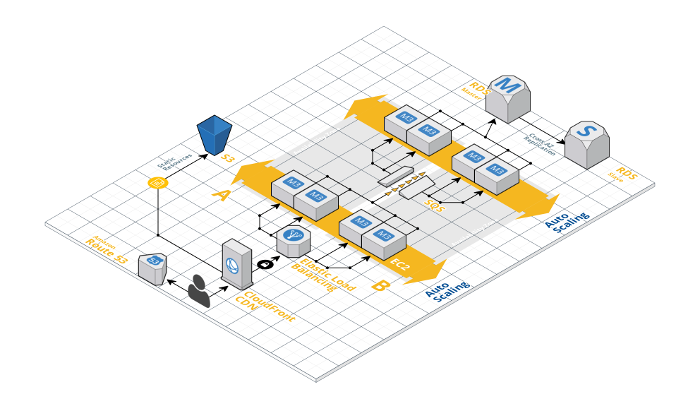
\includegraphics[width=0.8\textwidth]{resources/chapter-2-infrastructure-diagram.png}
%     \caption{Contoh gambar}
%   \end{figure}

%   \subsubsection{Subsubbab}

%   \blindtext

% \section{Studi Terkait}
% \blindtext
